\section{Comparativa SQL vs NoSQL}

\begin{wrapfigure}{L}{0.35\textwidth}
\vspace{-0.4cm}
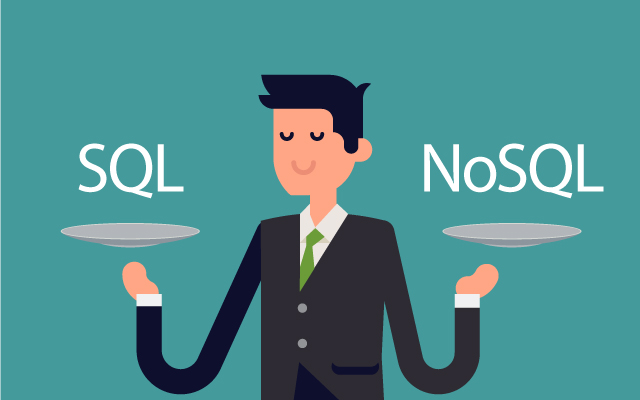
\includegraphics[width=0.3\textwidth]{images/sql_o_nosql}
\end{wrapfigure}

Las bases de datos no son para nada ajenas a las innovaciones y nuevas tendencias que se desarrollan a su alrededor. Es por ello que a las tradicionales bases SQL les salió ya hace ya un tiempo un competidor que cada vez tiene más fuerza, las bases NoSQL. Muchos desarrolladores han optado por migrar sus proyectos y trabajos a este modelo, pero para hacerlo es conveniente primero saber las diferencias entre ambas y también sus principales tecnologías, de forma que puedas tener información precisa sobre cuál conviene más en cada caso.

\begin{figure}[H]
	\centering
	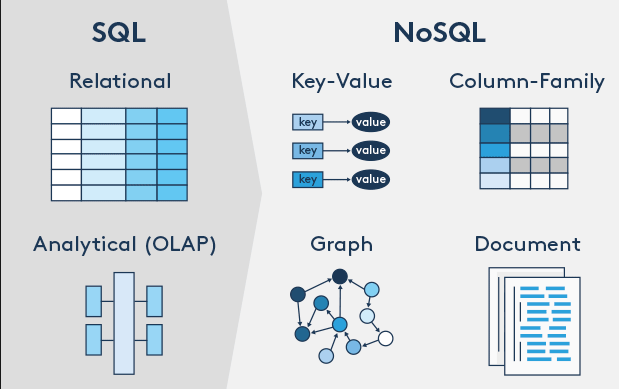
\includegraphics[scale=0.4]{images/comparativa_sql_vs_nosql}
	\caption{Comparativa SQL vs NoSQL}
\end{figure}

\subsection*{¿Cuándo utilizar qué tipo de base de datos?}

Entonces, ¿es NoSQL el sustituto directo para evolucionar de las antiguas bases de datos relacionales?. Esto no es cierto para todos los casos, sino que se tiene que tener en cuenta el diseño del problema para poder saber a qué modelo de base de datos se puede ajustar mejor.

A continuación se van a detallar las principales diferencias y contextos de uso.

\subsubsection*{Integridad de datos}

La integridad de datos es la garantía de que los datos almacenados mantendrán su exactitud y consistencia a través del tiempo. Tu código siempre deberá servir mientras tú mismo no modifiques su estructura.

\begin{itemize}

	\item \texttt{SQL:} Las tablas tienen estructuras rígidas, donde cada dato tiene un tipo definido, no podemos almacenar datos de otro tipo diferente, y no se vale más de un dato en un mismo campo. Puesto que todos los registros cumplen las mismas reglas, si tu código \textbf{funciona con un solo registro, servirá con todos los demás}.
	
	\item \texttt{NoSQL:} Hay varios tipos de base de datos NoSQL, pero en general, ninguna te exige que definas el tipo de datos que vas a almacenar. Un día un campo puede ser un número y al otro día un String o Array o hasta un JSON. Más que saber qué es la data, NoSQL pone mayor prioridad en cómo acceder dicha data.

\end{itemize}

\textsc{¿Qué significa esto?}

Que si necesitas que tus datos se mantengan \textbf{exactos y consistentes} a través del tiempo, \textbf{una base de datos SQL te lo garantiza}. Esto es lo ideal en muchos sistemas intolerantes a las fallas, donde mientras menos aberturas dejes, mejor (por ejemplo la mayoría, quizá totalidad, del software bancario y empresarial). Aquí SQL te cuida las espaldas.

Pero también, que si tus estructuras de datos son propensas a cambiar, el SQL te puede perjudicar al imponer una estructura rígida (por ejemplo, si estas en las fases de prototipo o lanzamiento temprano de una app, donde los datos que guardas son más maleables).

Mientras que \textbf{añadir llaves nuevas a un documento NoSQL suele ser muy fácil}, modificar tablas SQL puede traer muchos inconvenientes si ya el sistema funciona con cierta estructura, y más aún si hablamos de introducir cosas como llaves primarias.

\subsubsection*{Operaciones atómicas}

Una operación atómica es cuando haces un cambio que afecta a \textbf{múltiples entidades de la base de datos al mismo tiempo}. Esto suele acompañarse con el concepto de “transacciones”: decirle a la BD que, o cambian todas las tablas que queremos al mismo tiempo, o no cambia nada y la base de datos queda intacta (el famoso “rollback”, todo o nada).

\begin{itemize}

	\item \texttt{SQL:} Las bases de datos relacionales tienen atomicidad gracias a que sus tablas están conectadas y pueden “ponerse de acuerdo” para no aceptar cambios nuevos hasta que termine una transacción.
	
	Si tu sistema posee operaciones donde necesitas cambiar datos de varias entidades al mismo tiempo, ya es una alerta roja para usar SQL, pues estás reconociendo que hay relaciones entre los datos, y que éstas son importantes.
	
	Si además hablamos de \textbf{operaciones delicadas} (como procesar una factura, donde se suelen actualizar más cosas, por ejemplo el stock de un producto), es casi seguro que la atomicidad te salvará el pellejo de situaciones como que dos personas traten de pagar por el último de un producto al mismo tiempo.

	\item \texttt{NoSQL:} Datos no relacionales = no hay relaciones sobre las que hacer una transacción atómica. Simplemente, cuando quieres hacer cambios en 5 entidades diferentes, de frente o detrás de cámaras habrá 5 llamadas diferentes a la base de datos una detrás de otra.

\end{itemize}

\textsc{¿Qué significa esto?}

\texttt{NoSQL} no cuenta con \textbf{atomicidad}, y ésta \textbf{es vital para ciertos sistemas}.

¿La desventaja? \textbf{La atomicidad no es barata para la máquina}, consume capacidad de procesamiento y afecta el rendimiento de la base de datos, pues ésta hace el trabajo sucio para garantizar que nadie más se entrometa en una transacción.

¿Cuándo elegir \texttt{NoSQL}? \textbf{La atomicidad no siempre es crucial}.

Comparado con una inconsistencia en un estado de cuenta bancaria, ¿qué tan crítico es si dos usuarios difieren en la cantidad de likes de un post? \textbf{A veces la velocidad de respuesta es más importante} que la consistencia de datos (muchas app móviles caen en esto), y aquí brilla NoSQL.	

\subsubsection*{Escalabilidad}

Este suele ser un punto controversial cuando hablamos de cantidad de registros que podemos almacenar antes que la BD empiece a dar problemas. ¿La realidad? \textbf{Depende totalmente de la base de datos específica que usemos}.

Para empezar, cuando pensamos en escalabilidad es muy probable que realmente pensemos en \textbf{escalabilidad vertical}: aumentar el poder de una máquina para que pueda aguantar una mayor cantidad de datos.

Soluciones SQL como MySQL, Microsoft SQL Server y Postgre han probado su poder de escalar verticalmente a través de los años, pero NoSQL también tiene sus jugadores como Hadoop o Riak que, en sus respectivos campos (Big Data y soluciones distribuidas) aguantan datos como una montaña aguantando gotas de lluvia.

¿Entonces, donde hay mayor diferencia? En la \textbf{escalabilidad horizontal}, es decir, en cuántas máquinas diferentes podemos dividir la BD para repartir la carga.

\begin{itemize}

	\item \texttt{SQL:} La verdad es que la mayoría de soluciones SQL tienen buen soporte para escalar verticalmente.
	
	Pero cuando tratas de que la información en tu base de datos se mantenga consistente para todos los usuarios, los problemas llegan al hablar de miles y millones de registros. Aun con una máquina muy potente, puedes verte obligado a dividir tu base de datos entre diferentes procesadores y hasta servidores.
	
	Ahora, las bases de datos distribuidas SQL no son un concepto nuevo y compañías como Microsoft llevan años trabajando en ello, pero no es algo barato (para el bolsillo ni para el procesamiento).
	
	\textbf{Siempre hay cierto riesgo de presentar inconsistencias}, pues la BD ahora debe revisar que todo este en orden a través de diferentes máquinas.

	\item \texttt{NoSQL:} Cuando no tienes la consistencia de datos como prioridad, \textbf{distribuir y replicar} tu base de datos en múltiples máquinas \textbf{es trivial}, y por eso se considera que el NoSQL es excelente para bases de datos necesitan escalar horizontalmente (por ejemplo, en Big Data, donde una sola máquina se queda corta sumamente rápido).

\end{itemize}

\textsc{¿Qué significa esto?}

Las bases de datos relacionales ya vienen equipadas para crecer verticalmente, lo cual es más que suficiente para empresas pequeñas a grandes, proyectos personales, blogs y demás… hasta cierto punto, y mientras tengas \textbf{una buena máquina con la capacidad requerida}.

\texttt{NoSQL}, por el contrario, la tiene más fácil residiendo en \textbf{muchas máquinas menos potentes}.

\subsubsection*{Velocidad}

Esto es que tan rápidas son las lecturas y escrituras a la BD. Una necesidad básica, pero tan importante que \texttt{puede definir por sí sola con qué modelo nos quedamos}.

\begin{itemize}


\item \texttt{SQL:} Las garantías que te dan las relaciones conllevan un precio. Esto es más evidente cuando empezamos a hacer consultas con “joins” (que involucran múltiples entidades) y de repente una búsqueda \textbf{puede tardar minutos y hasta horas} debido a la gran cantidad de datos que está revisando.

Es un problema que se suele aliviar con buen diseño de la BD, pero está ahí y te morderá tarde o temprano.

\item \texttt{NoSQL:} Mientras que un buen diseño en SQL sirve para amortiguar un golpe, en NoSQL determinará que tanto jugo le saques a la velocidad con que viene.

Asumiendo que buscas tus datos de una sola entidad, las bases de datos no relacionales suelen contar con mecanismos de \textbf{búsqueda sumamente rápida} para conseguir un dato específico entre millones.

\end{itemize}

\textsc{¿Qué significa esto?}

Que si sabes cómo diseñar tu base de datos, es casi seguro que \textbf{una NoSQL bien diseñada gane por mucho en velocidad} a una SQL, haciéndolas sumamente atractivas para aplicaciones modernas donde los usuarios viven de su plan de datos, y donde si tu app no carga en un par de segundos ya piensan en desinstalar.

Siempre puedes optimizar ambos modelos hasta obtener un rendimiento aceptable, pero en NoSQL puedes \textbf{diseñar tu base de datos en función a las consultas que harás}, dándole una ventaja descomunal.


\subsubsection*{Consistencia vs redundancia}

Probablemente la diferencia más marcada entre ambos modelos, y donde más fácil nos es dejarnos llevar por nuestros conocimientos de SQL.

\begin{itemize}
\item \texttt{SQL:} La consistencia de datos es asegurarse de que un único dato este \textbf{una única vez en toda la base de datos}; y se suele lograr con el proceso de “Normalización” (reducir la cantidad de datos “repetidos” en la BD).

Esto garantiza que por ejemplo, si buscas el nombre de alguien, el nombre que verás es exactamente el mismo que podrían ver tu vecino o alguien en Pekín, si están conectados a la misma base de datos. Igual de importante, significa que mientras vayas navegando en tu app, si 10 pantallas diferentes cargan un dato, las 10 veces será el mismo dato.

\item \texttt{NoSQL:} La redundancia es repetir adrede los datos a conveniencia en varias partes de la BD (datos “de-normalizados”).

Por ejemplo, si almacenamos datos de una reservación hotelera, guardamos todos los datos de una persona en la entidad “Persona”. Pero además, guardamos una copia del nombre, teléfono y demás información personal en cada “Reservación” y posiblemente en cada “Factura” de esta persona.

Si cambian los datos de una persona en “Persona”, no necesariamente se reflejará este cambio en las otras entidades (ya esto queda a mano y decisión tuya); pero también hace que al buscar facturas o reservaciones, no tenemos que dar vueltas extra para obtener los datos de la persona.

\end{itemize}

\textsc{¿Qué significa esto?}

Algunas aplicaciones necesitan consistencia de datos, pero otras \textbf{prefieren el incremento en velocidad}. Recuerda que el espacio de almacenamiento es barato y solo se abarata más cada año, pero el procesamiento y los datos móviles aún son oro para los usuarios finales.

También, al diseñar bases de datos NoSQL, debes tener siempre en mente que \textbf{la redundancia está de tu lado}. Muchas veces nos quejamos al utilizar servicios como la Realtime Database de Firebase pues restringen nuestra capacidad para consultar diferentes colecciones (entidades) al mismo tiempo.

En realidad, están diseñados así para optimizar las consultas rápida, y el problema más común es que no aprovechamos al máximo la redundancia para poner la información que necesitamos en un único lugar.

\subsubsection*{Comodidad para el desarrollador}

\begin{itemize}


\item \texttt{SQL:} La comunidad SQL \textbf{lleva décadas madurando}, y esto se traduce no solo en mejores herramientas administrativas, sino en estándares mejores definidos, mayor documentación, y hasta comunidades más grandes de desarrolladores listos para ayudarte con tus problemas o unirse a tu equipo de trabajo.

\item \texttt{NoSQL:} Lo pondré así, buena suerte consiguiendo herramientas administrativas como phpMyAdmin y de manera gratuita. Aquí el punto fuerte es la conveniencia: factores como que los datos no necesiten tipos o que puedas aprovechar la redundancia, hacen \textbf{más flexible} el desarrollar con NoSQL.

Si estás prototipando, \textbf{los cambios son más rápidos y tienen menos consecuencias}. Si sabes qué quieres mostrar a tus usuarios, es fácil diseñar bases de datos especializadas en servir exacta y rápidamente la información que quieres.

\end{itemize}

\textsc{¿Qué significa esto?}

Que las base de datos \textbf{NoSQL te suelen dar más libertad para experimentar y equivocarte}, haciendo cambios a diestra y siniestra… pero éstas son necesidades que no tendrás siempre.

\textbf{Cuando tienes un sistema mejor definido}, te hará falta contar con buenas herramientas administrativas o saber que hay más gente ahí afuera lista para apoyarte o unirse a tu equipo rápidamente, y en esto \textbf{SQL brilla}.

En resumen, se puede decir que \textbf{NoSQL} te da más facilidades como desarrollador y \textbf{ventajas a corto plazo}, mientras que los beneficios de \textbf{SQL} los sueles ver cuando va pasando el tiempo y te toca \textbf{mantener el sistema}.

\vspace{1cm}

\begin{table}[H]
	\centering
	\begin{tabular}[c]{|l |l |l|}
		\hline
		\rowcolor{azulOscuro} \color{white}Característica & \color{white}NoSQL & \color{white}SQL \\
		\hline
		\cellcolor{azulClaro} Rendimiento & \cellcolor{verdeSuave}Alto & \cellcolor{rojoSuave}Bajo \\
		\cellcolor{azulClaro}Confiabilidad & \cellcolor{rojoSuave}Baja & \cellcolor{verdeSuave}Buena \\
		\cellcolor{azulClaro}Disponibilidad & \cellcolor{verdeSuave}Buena & \cellcolor{verdeSuave}Buena \\
		\cellcolor{azulClaro}Consistencia & \cellcolor{rojoSuave}Baja & \cellcolor{verdeSuave}Buena \\
		\cellcolor{azulClaro}Almacenamiento & \cellcolor{verdeSuave}Soporta enormes cantidades & \cellcolor{amarilloSuave}Cantidades medio/grande \\
		\cellcolor{azulClaro}Escalabilidad & \cellcolor{verdeSuave}Alta & \cellcolor{amarilloSuave}Alta pero más cara \\
		\hline
	
	\end{tabular}
	\caption{Resumen de las características NoSQL y SQL}
\end{table}


\newpage